\documentclass[11pt]{article}
\usepackage[french]{babel}
\usepackage[utf8]{inputenc}
\usepackage[T1]{fontenc}
\usepackage{geometry}
\geometry{hmargin=2cm,vmargin=2cm}
\usepackage{eucal}
\usepackage{colortbl}
\usepackage{lscape}
\usepackage{amssymb}
\usepackage{amscd} 
\usepackage{amsfonts,amsmath,amsthm,amssymb,stmaryrd,eurosym} 
\usepackage{textcomp}
\usepackage{icomma}
\usepackage{calrsfs}
\usepackage{fancyhdr}
\usepackage{listings}
\usepackage{makecell}
\usepackage{appendix}
\usepackage{graphicx}
\renewcommand{\v}[1]{\overrightarrow{#1}}
\usepackage[svgnames,dvipsnames]{xcolor}
\newcommand{\fboxb}[1]{\fbox{\color{blue}#1\color{black}}}
\renewcommand{\b}[0]{$\bullet$}
\usepackage{tcolorbox}
\usepackage{dirtree}
\usepackage{tikz}
\usetikzlibrary{arrows.meta}
\usepackage{algorithm,algorithmic}
\usepackage{appendix}
\usepackage{hyperref}

\definecolor{codegreen}{rgb}{0,0.6,0}
\definecolor{codegray}{rgb}{0.5,0.5,0.5}
\definecolor{codepurple}{rgb}{0.58,0,0.82}
\definecolor{backcolour}{rgb}{0.95,0.95,0.92}

\lstdefinestyle{mystyle}{
    backgroundcolor=\color{backcolour},   
    commentstyle=\color{codegreen},
    keywordstyle=\color{magenta},
    numberstyle=\tiny\color{codegray},
    stringstyle=\color{codepurple},
    basicstyle=\ttfamily\footnotesize,
    breakatwhitespace=false,         
    breaklines=true,                 
    captionpos=b,                    
    keepspaces=true,                 
    numbers=left,                    
    numbersep=5pt,                  
    showspaces=false,                
    showstringspaces=false,
    showtabs=false,                  
    tabsize=2,
    inputencoding=utf8,
    literate        =
                        {é}{{\'e}}{1}%
                        {è}{{\`e}}{1}%
}

\lstset{style=mystyle}

\lstdefinestyle{mybashstyle}{
  language=bash,
  basicstyle=\ttfamily\footnotesize,
  commentstyle=\color{gray},
  keywordstyle=\color{blue},
  stringstyle=\color{red},
  tabsize=4,
  frame=single,
  numbers=left,
  numberstyle=\tiny\color{gray},
  backgroundcolor=\color{gray!5},
  captionpos=b,
  belowcaptionskip=4pt
}

\lstdefinestyle{mycstyle}{
  language=C,
  basicstyle=\ttfamily\footnotesize,
  showstringspaces=false,
  commentstyle=\color{green!40!black},
  keywordstyle=\color{blue},
  stringstyle=\color{red},
  tabsize=4,
  frame=single,
  numberstyle=\tiny\color{gray},
  backgroundcolor=\color{gray!5},
  captionpos=b,
  belowcaptionskip=4pt
}


\title{PCL1}
\author{GIANELLI Thomas}
\date{\today}
\begin{document}
\thispagestyle{empty}
\vspace*{-1.5cm}

\hspace{-1.5cm}
\includegraphics[scale=0.2]{logo_tn.jpg}
	
\vspace*{-1.6cm}
	
\hspace{13.5cm}
\includegraphics[scale=0.2]{logo_ul.png}



\vspace*{5cm}	% Espacement vertical
\begin{center}	% On centre le texte
{\Huge \bf Projet Compilation \\\vspace{0.2cm} }	% \huge fait que le texte est gros, \bf fait que le texte est gras
\vspace{3cm}
\Large Partie I \\
\vspace{3cm}
Travail réalisé par AGRA Maxence, BEKHEDDA Maxence, DÉCAVÉ Gabriel et GIANELLI Thomas
\vfill	% On va jusqu'au bas de la page avant de mettre le texte ci-dessous
\today
\end{center}
\newpage


\tableofcontents
\newpage

\section{Introduction}

Le but de cette première partie du projet est la construction d'un arbre abstrait à partir d'un code écrit en \texttt{canAda}. 

Pour ce faire, il nous faut dans un premier temps un analyseur lexical nous permettant de transformer notre code qui est un simple fichier \texttt{txt} en une suite de tokens. Ensuite, vient l'étape de l'analyse syntaxique. Cela nécessite la construction d'une grammaire pour vérifier que notre code est bien une succession de règles valides. Enfin, une fois que nous avons toutes nos règles, nous pouvons construire l'arbre de dérivation puis l'arbre abstrait de notre code et le visualiser.

Nous avons choisi d'utiliser \texttt{python} pour la réalisation de ce projet. D'une part, il s'agit du langage que nous maîtrisons le mieux tous les quatre, et d'autre part nous estimons que c'est celui qui offre le plus de liberté grâce à la simplicité des structures et au nombre de bibliothèques disponibles.

\section{Analyse Lexicale}

Pour commencer, nous avons codé un analyseur lexical \texttt{lexeur\_non\_automate.py} en utilisant les regex. Nous avons également créé une liste \texttt{lexique.txt} contenant les mots-clés afin de les différencier aisément des noms de variable, ainsi qu'une liste avec les opérateurs du langage car il n'existe pas de regex qui nous renvoie uniquement ceux-là.

Nous supprimons ensuite les commentaires et les tokens de saut de ligne. Nous les avions gardés jusqu'à présent, car ils nous permettaient de savoir à quelle ligne se trouvait l'erreur si notre analyseur lexical détectait une erreur lexicale.

Enfin, nous affectons à chaque variable un entier. Ce code nous permettra de manipuler plus facilement nos variables par la suite.

Nous avons donc ainsi transformé notre fichier \texttt{txt} d'entrée en une liste de nombres et de tuples. Chacun de ses éléments est un token dont on peut retrouver la valeur en se référant au lexique et au code lexical générés à l'exécution.

\section{Analyse Syntaxique}

L'analyse syntaxique commence par la création d'une grammaire efficace et respectant les priorités opératoires (voir annexe \hyperref[tab:priorities]{Table des priorités}). En effet, une grammaire nous est donnée dans le sujet, mais celle-ci n'est pas LL(1). Le caractère LL(1) d'une grammaire permet de savoir quelle règle appliquer après la lecture d'un token.
Notre premier objectif a donc été de rendre la grammaire LL(1) au plus d'endroits possibles tout en respectant les priorités opératoires. Pour ce fait, nous avons donc ajouté de nombreuses règles afin d'obtenir une grammaire (jointe en annexe \ref{Grammaire}) qui respecte les priorités opératoires et qui est LL(1) en dehors d'un cas dans INSTR. 

\subsection{Construction de l'arbre de dérivation}

Après avoir modifié la grammaire, nous avons créé la table d'analyse LL. Cette table permet de savoir quelle règle appliquée. Nous avons donc codé une fonction pour chaque règle de grammaire en lisant cette table d'analyse LL. Ces fonctions sont dans le dossier \texttt{Analyse syntaxique/Arbre}. Pour générer l'arbre, nous donnons la liste de tokens à la règle de l'axiome \texttt{FICHIER}. Puis par récursivité, la fonction consomme les tokens et ajoute les noeuds à l'arbre. 
Pour afficher l'arbre, nous utilisons le module \texttt{digraph} de la bibliothèque \texttt{graphviz}. 

\subsection{Construction de l'arbre abstrait}

La construction de l'arbre abstrait correspond à élaguer l'arbre de dérivation en supprimant les branches successives inutiles ainsi que les feuilles non terminales et à remonter les opérateurs en respectant les règles d'associativité. 

\section{Difficultés rencontrées}

Initialement, nous avions l'intention de créer un analyseur lexical qui fonctionne comme un automate. Cependant, nous avons changé d'approche car il était plus simple d'utiliser des règles de regex pour parser le fichier et récuperer la liste de tokens.

Il nous a fallu ensuite modifier la grammaire pour essayer de la rendre LL(1) au plus d'endroits possible afin de pouvoir l'utiliser dans l'analyseur syntaxique. Comme nous n'avions pas anticipé la gestion des priorités opératoires, nous avons dû voir la grammaire une seconde fois.

Enfin, nous ne pouvions pas voir les erreurs dans la grammaire avant d'afficher un bon arbre de dérivation voir même un arbre abstrait. Quand nous avons réussi à élaguer efficacement l'arbre, il était plus simple de voir les erreurs de grammaire. 

\section{Répartition et temps passé sur chaque tâche}

Le tableau \ref{tab:exemple} en annexe présente la répartition des tâches avec l'estimation de temps passée par chacun sur chaque tâche réalisée.

\section{Conclusion}

Pour conclure, le projet de compilation a été particulièrement exigeant surtout la transformation de la grammaire LL(1). Cependant, ce projet a montré l'importance de la théorie dans la réalité du développement logiciel et a offert une perspective approfondie sur la création d'un compilateur. 
Notre projet prend en compte les priorités opératoires et l'associativité. Nous essayons d'afficher le maximum d'informations quand nous détectons une erreur, mais notre programme ne continue pas toujours. 
Pour finir, nous avons aussi apprécié la mise pratique de ce que nous avons appris durant les modules de Théories des langages et de Traduction 1. Ce projet fut motivant et instructif. 

\newpage

\begin{appendix}

\section{Priorités opératoires et associativités}
\label{tab:priorities}

    \begin{table}[h]
        \centering
        \begin{tabular}{|c|c|c|}
            \hline
            opérateur & associativité & précédence \\
            \hline
            \textit{or, or else} & gauche & plus faible \\
            \hline
            \textit{and, and then} & gauche & \\
            \hline
            \textit{not} & & \\
            \hline
            \textit{= /=} & & \\
            \hline
            \textit{> >= < <=} & & \\
            \hline
            \textit{+ -} & gauche & \\
            \hline
            \textit{* / rem} & gauche & \\
            \hline 
            \textit{- (unaire)} & & \\
            \hline
            \textit{.} & gauche & plus forte \\
            \hline
        \end{tabular}
        \caption{Table des priorités opératoires et de l'associativité des opérateurs}
    \end{table}



\section{La grammaire}\label{Grammaire}

\begin{lstlisting}[caption={La grammaire que nous avons obtenue}]
FICHIER -> with IDENT point text_io pointvirgule use ada point text_io pointvirgule procedure IDENT is DECLETOILE begin INSTRPLUS end IDENTINTER pointvirgule eof .

IDENT -> ident .
IDENTPLUS -> IDENT IDENTPLUS2 .
IDENTPLUS2 -> virgule IDENT IDENTPLUS2 | .
IDENTINTER -> IDENT | . 

DECL -> type IDENT DECL1 
        | IDENTPLUS deuxpoints TYPE ASSIGNINTER pointvirgule 
        | procedure IDENT PARAMSINTER is DECLETOILE begin INSTRPLUS end IDENTINTER pointvirgule
        | function IDENT PARAMSINTER return TYPE is DECLETOILE begin INSTRPLUS end IDENTINTER pointvirgule.
DECL1 -> pointvirgule | is DECL2 .
DECL2 -> access IDENT pointvirgule | record CHAMPSPLUS end record pointvirgule .

DECLETOILE -> DECL DECLETOILE2 | .
DECLETOILE2 -> DECL DECLETOILE2 | .

CHAMPS -> IDENTPLUS deuxpoints TYPE pointvirgule.

CHAMPSPLUS -> CHAMPS CHAMPSPLUS2 .
CHAMPSPLUS2 -> CHAMPS CHAMPSPLUS2 | .

TYPE -> IDENT | access IDENT .

PARAMS -> ( PARAMPLUS ) .
PARAMSINTER -> PARAMS | .
PARAM -> IDENTPLUS deuxpoints MODEINTER TYPE .
PARAMPLUS -> PARAM PARAMPLUS2 .
PARAMPLUS2 -> pointvirgule PARAM PARAMPLUS2 | .

MODE -> in MODE2 .
MODE2 -> out | .

MODEINTER -> MODE | .

EXPR -> OP EXACCES .
EXPR1 -> ENTIER | CARACTER | true | false | null | ( EXPR ) | IDENT EXPR2 | new IDENT | character'val ( EXPR ).
EXPR2 -> EXPRPLUS | .
EXACCES -> point IDENT EXACCES | .

EXPRINTER -> EXPR | .

EXPRPLUS ->  ( EXPR EXPRPLUS2 ) .
EXPRPLUS2 -> virgule EXPR EXPRPLUS2 | .

INSTR -> OP point IDENT INSTR2
        | IDENT INSTR2
        | return EXPRINTER pointvirgule 
        | begin INSTRPLUS end pointvirgule 
        | while EXPR loop INSTRPLUS end loop pointvirgule 
        | if EXPR then INSTRPLUS ELSIFETOILE ELSEINTER end if pointvirgule 
        | for IDENT in REVERSEINTER EXPR point point EXPR loop INSTRPLUS end loop pointvirgule.

INSTR2 -> deuxpoints eg EXPR pointvirgule 
        | pointvirgule 
        | EXPRPLUS pointvirgule.

INSTRPLUS -> INSTR INSTRPLUS2.
INSTRPLUS2 -> INSTRPLUS | .

REVERSEINTER -> reverse | .

OP -> OPE1 OPE' .
OPE' -> or ELSE OPE1 OPE' | .
OPE1 -> OPE2 OPE1' .
OPE1' -> and THEN OPE2 OPE1' | .
OPE2 -> OPE3 OPE2' .
OPE2' -> not OPE3 OPE2' | .
OPE3 -> OPE4 OPE3' .
OPE3' -> COMPARATEUR OPE4 OPE3' | .
OPE4 -> OPE5 OPE4'.
OPE4' -> ORDRE OPE5 OPE4' | .
OPE5 -> OPE6 OPE5'.
OPE5' -> ADD OPE6 OPE5' | .
OPE6 -> OPE7 OPE6' .
OPE6' -> MULT OPE7 OPE6' | .
OPE7 -> moins OPE8 | OPE8 .
OPE8 -> EXPR1 .

ELSE -> else | .
THEN -> then | .
COMPARATEUR -> eg | dif .
ORDRE -> inf EGAL | sup EGAL .
EGAL -> eg | .
ADD -> plus | moins .
MULT -> fois | div | rem .

ELSEINTER -> else INSTRPLUS | .
ELSIFETOILE -> elsif EXPR then INSTRPLUS ELSIFETOILE | .
ASSIGNINTER -> deuxpoints eg EXPR | .
ENTIER -> entier .

CARACTER -> caracter .
\end{lstlisting}
	
\newpage

\section{Répartition et temps passé sur chaque tâche}

    \begin{table}[h]
        \centering
        \begin{tabular}{|c|c|c|c|c|}
            \hline
            Tâches réalisées & Maxence A. & Maxence B. & Gabriel & Thomas \\
            \hline
            Création de l'analyseur lexical & / & 8h & 4h & 10h \\
            Tests de l'analyseur lexical & / & 2h & / & 2h \\
            Modification de la grammaire & 4h & 6h & 4h & 4h  \\
            Gestion des opérateurs de la grammaire & 2h & 6h & 2h & 4h \\
            Création des fonctions pour l'arbre de dérivation & 8h & 16h & 8h & 8h \\
            Création des fonctions pour l'arbre abstrait & 6h & / & 6h & 10h \\
            Création des tests & 1h & 2h & 1h & 1h \\
            Rédaction du rapport & 4h & 1h & 1h & 2h \\
            \hline
        \end{tabular}
        \caption{Répartition et temps passé sur chaque tâche}
        \label{tab:exemple}
    \end{table}

\section{Exemple}

\subsection{Le code}

\begin{lstlisting}[caption={Code d'un programme de test}]
with Ada.Text_IO ; use Ada.Text_IO ;

procedure MonFichier is
begin
   if (X = 0) then
      i := 3*4/2;
   elsif not (X = 1) then
      i := 2;
   else
      i := 3;
   end if;
end MonFichier;

\end{lstlisting}


\vspace{0.5cm}

\subsection{L'arbre généré}
\begin{figure}[H]
	\hspace{-0.7cm} 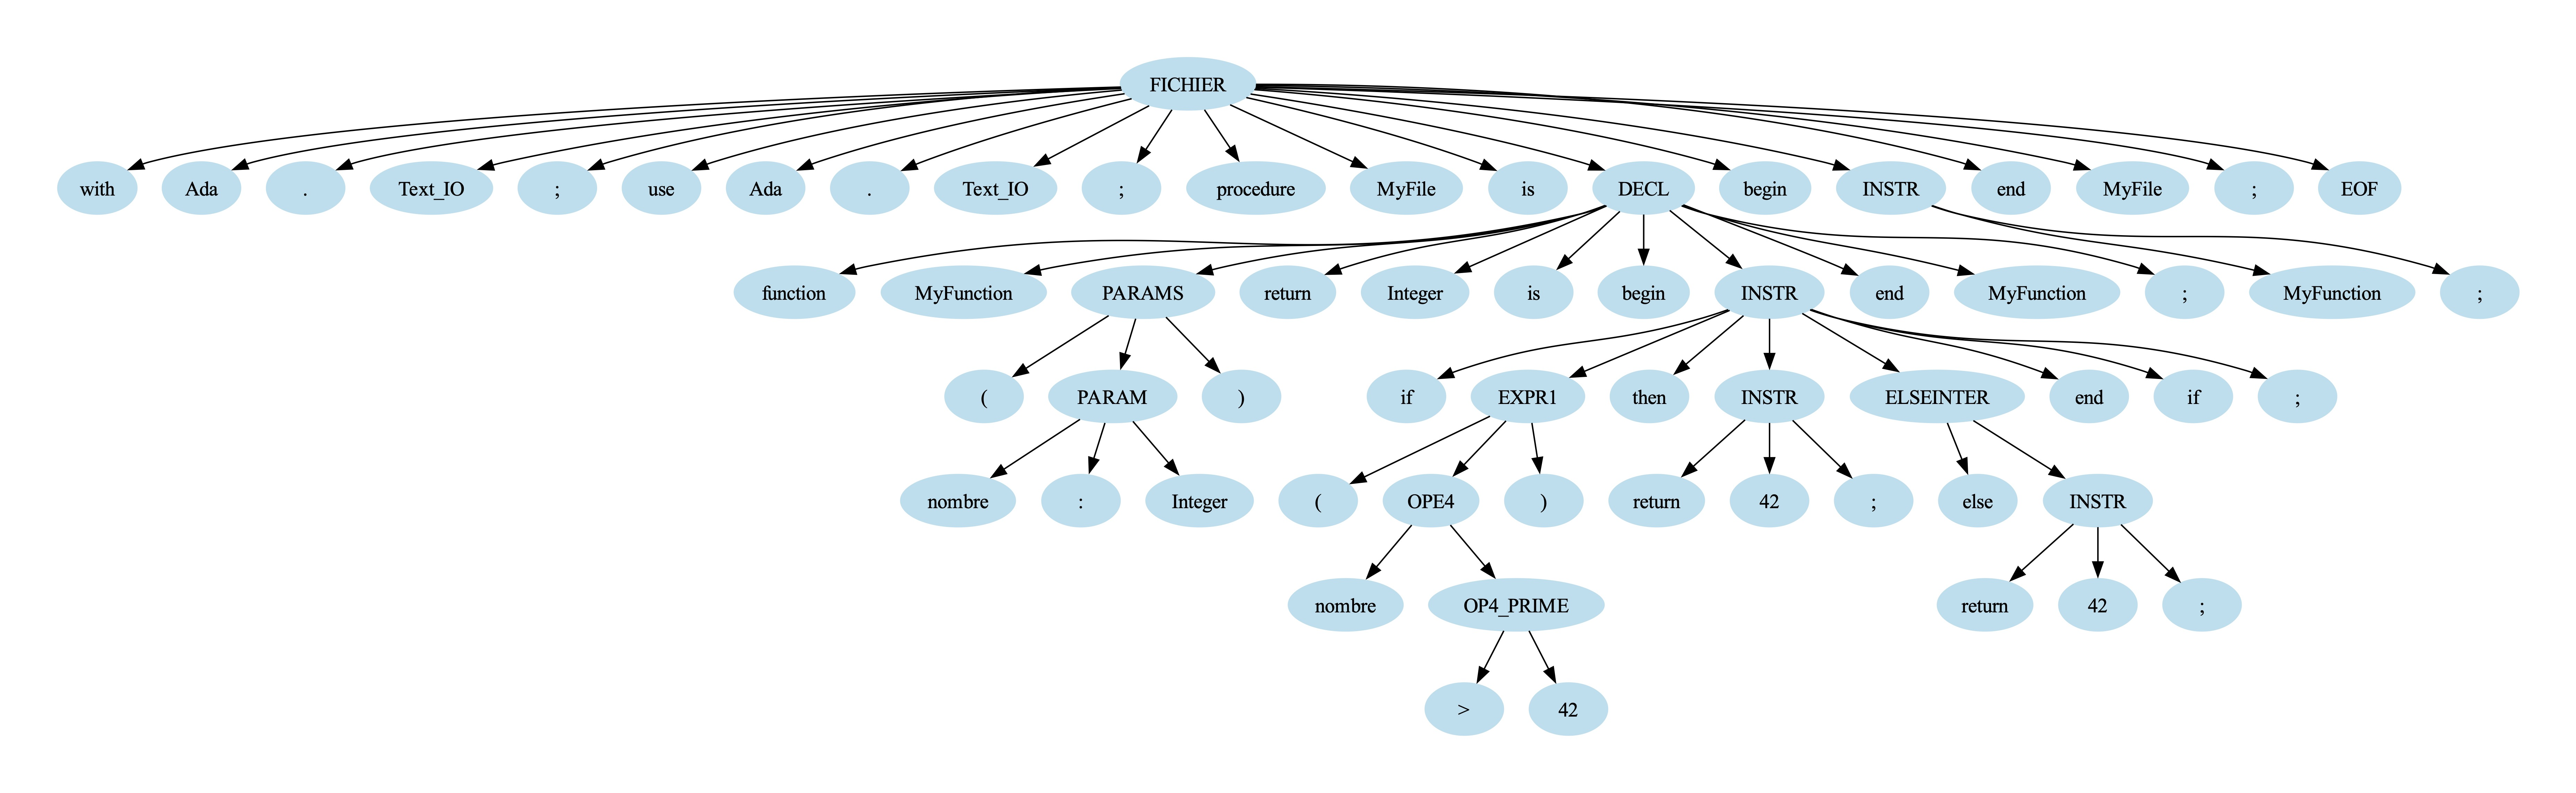
\includegraphics[scale=0.27]{arbre.pdf}
	\caption{Arbre généré lors de l'exécution de notre programme sur le code précédent}
	
\end{figure}

\end{appendix}


\end{document}

